\chapter{Clasificación de los grupos de alumnos según su rendimiento}\label{sec:chapterXIII}
\addcontentsline{toc}{chapter}{Clasificación de los grupos de alumnos según su rendimiento}

Para realizar la identificación de los subconjuntos de alumnos definidos en la Sección \ref{sec:badstudents}, se empleará el algoritmo de clasificación de Quinlan C5.0 \cite{Quinlan:See5C5}, que no es más que una herramienta de aprendizaje supervisado que genera un árbol de decisión o un conjunto de reglas. Así pues, las distintas categorías en las que se clasificarán a los grupos vendrán dadas en las hojas de dichos árboles y en los consecuentes de las reglas respectivamente. El clasificador estadístico C5.0 se basa en el concepto de entropía, seleccionando primero aquellas características cuyos valores se diferencian más entre diferentes categorías de grupos de alumnos.

Se utilizarán como variables de entrada del clasificador tanto las medidas clásicas de rendimiento presentadas en el Capítulo \ref{chapter:rendimiento} como las medidas grafo-teóricas (Sección \ref{sec:complexity}). Por su parte, como categorías de salida, tendremos tanto una única partición en alumnos ``LOW'', que se supone que requieren más esfuerzo para superar el laboratorio, como las cinco particiones que se muestran en la Figura \ref{fig:KMeans5}.

Dado que hay muy pocos registros ($77$ en cada nivel), el problema de clasificación va a ser difícil, y, con el fin de aumentar las evidencias requeridas por C5.0 para trabajar, el conjunto de datos se agrupará cada tres niveles consecutivos. Así pues, por un lado, agruparemos los niveles $3$, $4$ y $5$ para realizar predicciones al principio de la práctica y, por otro lado, agruparemos los niveles $8$, $9$ y $10$. Así pues, las siguientes secciones se dividrán en dos subapartados, dependiendo de la parte del dataset que estemos utilizando para entrenar el clasificador.

\section{Clasificación empleando las métricas clásicas de rendimiento}



\section{Clasificación empleando las medidas de complejidad de propósito general}

\subsection{Clasificación empleando los niveles 3, 4 y 5}

El resultado es que C5.0 obtiene un conjunto de reglas capaz de clasificar exactamente los $35$ de los $36$ casos de grupos \emph{``LOW''} del nivel $3$ en adelante, es decir, a partir de un tercio del periodo de tiempo dedicado a la práctica, con un $p$ value $p = 3.843e-16$ estadísticamente muy relevante (Figura \ref{fig:cm2}). Además, las reglas obtenidas (Figura \ref{rules2}) tienen pleno sentido. Por ejemplo, la regla $7$ dice: ``Un grupo está en riesgo si está centrado en los problemas con numeración alta (\texttt{Be > 6})''. O la regla $3$ que dice ``Un grupo está en riesgo si no se ha centrado por igual en todos los problemas (\texttt{Ba > 3.366005}) y recorre caminos menos largos en media (\texttt{WDag > -4.317488}) teniendo en cuenta que el valor de máxima probabilidad de la métrica $WDag$ es $-4.19$.

\begin{figure}[H]
\centering
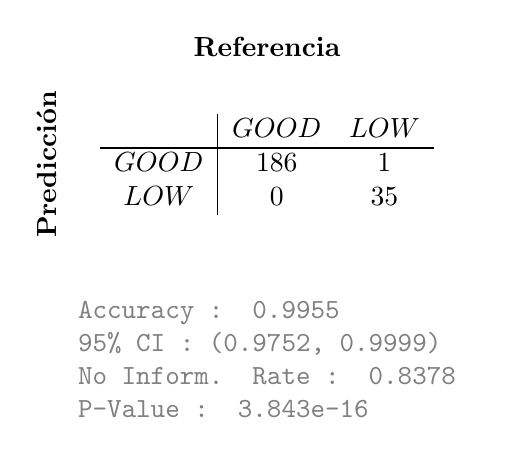
\begin{tikzpicture}
  \node (matrix)  {$\begin{array}{c|cc}
			 & GOOD & LOW \\ \hline
        GOOD & 186  & 1 \\
        LOW & 0 & 35
\end{array}$};
  \node[above of= matrix, node distance=0.5cm, yshift=1cm,font=\color{black}] {\textbf{Referencia}};
  \node[left of= matrix, node distance=3.5cm, rotate=90, anchor=center,yshift=-0.7cm,font=\color{black}] {\textbf{Predicción}};
  % Tabular environment for additional text
  \node[below of=matrix, node distance=2.5cm,font=\color{gray}]{
    \begin{tabular}{l}
      \texttt{Accuracy : 0.9955} \\
      \texttt{95\% CI : (0.9752, 0.9999)} \\
      \texttt{No Inform. Rate : 0.8378} \\
      \texttt{P-Value : 3.843e-16 }
    \end{tabular}
  };
\end{tikzpicture}
\caption{Aprendiendo a identificar a los grupos \emph{``LOW''}, es decir, aquellos con una puntuación inferior a una nota $8.1$ sobre $10$.}
\label{fig:cm2}
\end{figure}

\begin{tcolorbox}[title=Reglas de clasificación para identificar grupos de tipo \emph{``LOW''}.]
  %add special color box to list of listings
  \makeatletter
  \addcontentsline{lol}{subsection}{\kvtcb@title}
  \makeatother
\begin{multicols}{2}
    \begin{minted}{R}
Rule 11/1: (17.8, lift 1.5)
	Ba > 9.26712
	->  class GOOD  [0.949]

Rule 11/2: (200.7/68.3, lift 1.0)
	De > 0.0952381
	->  class GOOD  [0.658]

Rule 11/3: (8.5/0.3, lift 2.5)
	WDag > -4.317488
	Ba > 3.366005
	->  class LOW  [0.880]

Rule 11/4: (5, lift 2.4)
	Dm <= 1.2
	Ef <= 4
	St > 1.791759
	->  class LOW  [0.858]

Rule 11/5: (8.3/0.6, lift 2.4)
	De <= 0.0989011
	Ef <= 4
	Ba <= 9.26712
	->  class LOW  [0.850]

Rule 11/6: (9.4/1.1, lift 2.3)
	De > 0.1153846
	Ef > 3
	Ef <= 4
	WDag <= -6.612041
	Ba > 3.366005
	->  class LOW  [0.818]

Rule 11/7: (3.4, lift 2.3)
	Be > 6
	->  class LOW  [0.814]

Rule 11/8: (13.3/2.3, lift 2.2)
	De <= 0.0952381
	Ba <= 9.26712
	->  class LOW  [0.783]

Rule 11/9: (19.9/5.4, lift 2.0)
	Dm <= 1.222222
	Ef <= 3
	St > 0.6931472
	Ba <= 9.26712
	->  class LOW  [0.707]
    \end{minted}
  \end{multicols}
\label{rules2}
\end{tcolorbox}

Pero no sólo esto, ¿podríamos dar un gran paso y predecir no sólo equipos \emph{``LOW''}/\emph{``GOOD''}, sino también un límite inferior y superior de sus calificaciones finales, y adivinar en cuál de los $5$ intervalos de la Figura \ref{fig:KMeans5} se encuentran? La respuesta es, felizmente sí.

\subsection{Clasificación empleando los niveles 8, 9 y 10}


\section{Clasificación empleando una combinación de todas las métricas}

A continuación, se repetirán los experimentos anteriores, pero ahora empleando las funciones $s$, $p$, $Cl$, $De$, $Dm$, $Le$, $Di$, $We$, $Ef$, $St$, $Dag$, $WDag$, $Be$ y $Ba$.

\subsection{Clasificación empleando los niveles 3, 4 y 5}

El resultado es que C5.0 obtiene un conjunto de reglas capaz de clasificar exactamente los $36$ casos de grupos \emph{``LOW''} del nivel $3$ en adelante, es decir, a partir de un tercio del periodo de tiempo dedicado a la práctica, con un $p$ value $p < 2.2e-16$ estadísticamente muy relevante (Figura \ref{fig:cm1}). Entre las reglas obtenidas (Figura \ref{rules1}), la regla $6$ dice: ``Un grupo está en riesgo si ha realizado pocas sesiones (\texttt{s <= 21}) y el grafo no está lo suficientemente balanceado (\texttt{Ba > 3,366005})''. O la regla $7$ que dice ``Un grupo está en riesgo si tiene pocas sesiones \texttt{We <= 0.01620162} y no se centra por igual en todos los problemas \texttt{Ba > 3.366005}''. %Esto es como el mal gráfico mostrado al principio de este documento en la Figura 1, largo y desconectado.

\begin{figure}[H]
\centering
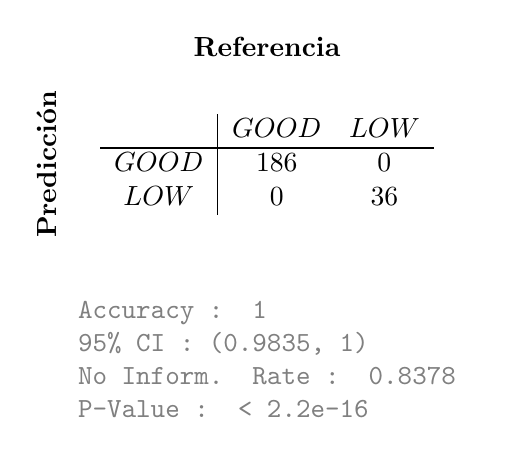
\begin{tikzpicture}
  \node (matrix)  {$\begin{array}{c|cc}
			 & GOOD & LOW \\ \hline
        GOOD & 186  & 0 \\
        LOW & 0 & 36
\end{array}$};
  \node[above of= matrix, node distance=0.5cm, yshift=1cm,font=\color{black}] {\textbf{Referencia}};
  \node[left of= matrix, node distance=3.5cm, rotate=90, anchor=center,yshift=-0.7cm,font=\color{black}] {\textbf{Predicción}};
  % Tabular environment for additional text
  \node[below of=matrix, node distance=2.5cm,font=\color{gray}]{
    \begin{tabular}{l}
      \texttt{Accuracy : 1} \\
      \texttt{95\% CI : (0.9835, 1)} \\
      \texttt{No Inform. Rate : 0.8378} \\
      \texttt{P-Value : < 2.2e-16}
    \end{tabular}
  };
\end{tikzpicture}
\caption{Aprendiendo a identificar a los grupos \emph{``LOW''}, es decir, aquellos con una puntuación inferior a una nota $8.1$ sobre $10$.}
\label{fig:cm1}
\end{figure}

\begin{tcolorbox}[title=Reglas de clasificación para identificar grupos de tipo \emph{``LOW''}.]
  %add special color box to list of listings
  \makeatletter
  \addcontentsline{lol}{subsection}{\kvtcb@title}
  \makeatother
\begin{multicols}{2}
    \begin{minted}{R}
Rule 5/1: (20.9, lift 1.5)
	s > 177
	Ba <= 5.651057
	->  class GOOD  [0.956]

Rule 5/2: (21.2/0.3, lift 1.5)
	s > 21
	Cl > 0.6111111
	WDag > -6.562621
	->  class GOOD  [0.945]

Rule 5/3: (11, lift 1.4)
	Ba <= 3.366005
	->  class GOOD  [0.923]

Rule 5/4: (41.2/4.6, lift 1.4)
	WDag <= -6.678342
	->  class GOOD  [0.871]

Rule 5/5: (143.1/44.1, lift 1.1)
	Cl <= 0.4866667
	->  class GOOD  [0.689]

Rule 5/6: (12.4, lift 2.6)
	s <= 21
	Ba > 3.366005
	->  class LOW  [0.931]

Rule 5/7: (10.3, lift 2.6)
	We <= 0.01620162
	Ba > 3.366005
	->  class LOW  [0.918]

Rule 5/8: (19/1.4, lift 2.5)
	s > 177
	s <= 271
	Cl <= 0.4866667
	WDag > -6.39693
	Ba > 5.651057
	->  class LOW  [0.885]

Rule 5/9: (9.8/0.6, lift 2.4)
	s <= 105
	Cl <= 0.6111111
	We > 0.1657658
	->  class LOW  [0.868]

Rule 5/10: (19.6/4.3, lift 2.1)
	WDag > -6.678342
	WDag <= -6.562621
	->  class LOW  [0.755]

Rule 5/11: (26.4/7.8, lift 1.9)
	Cl > 0.4866667
	Cl <= 0.6111111
	WDag > -6.678342
	Ba > 3.366005
	->  class LOW  [0.690]
    \end{minted}
  \end{multicols}
\label{rules1}
\end{tcolorbox}

\subsection{Clasificación empleando los niveles 8, 9 y 10}